% Lecture 1: the differential approach (the field at every point, seen through a fluid element)
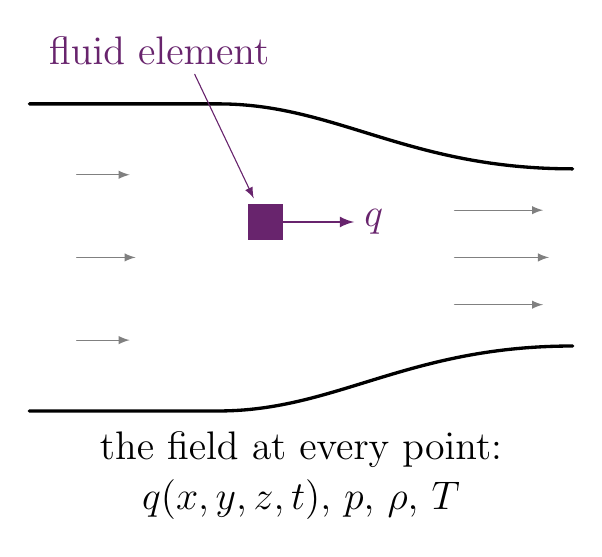
\begin{tikzpicture}[scale=1.5, >=latex, line cap=round]
  \definecolor{dpurple}{HTML}{68246D}
  \draw[very thick] (0,1.3) -- (1.6,1.3) .. controls (2.6,1.3) and (3.2,0.75) .. (4.6,0.75);
  \draw[very thick] (0,-1.3) -- (1.6,-1.3) .. controls (2.6,-1.3) and (3.2,-0.75) .. (4.6,-0.75);
  % a few local velocity vectors
  \foreach \x/\y/\l in {0.4/0.7/0.45, 0.4/0/0.5, 0.4/-0.7/0.45, 3.6/0.4/0.75, 3.6/-0.4/0.75, 3.6/0/0.8}
    \draw[->, gray] (\x,\y) -- ++(\l,0);
  % fluid element
  \fill[dpurple] (1.85,0.15) rectangle (2.15,0.45);
  \draw[->, thick, dpurple] (2.15,0.3) -- (2.75,0.3) node[right, font=\Large] {$\vect{q}$};
  \node[dpurple, font=\Large] (fe) at (1.1,1.75) {fluid element};
  \draw[dpurple, ->] (fe.south) ++(0.3,0) -- (1.9,0.5);
  \node[font=\Large, align=center] at (2.3,-1.85) {the field at every point:\\ $\vect{q}(x,y,z,t)$, $p$, $\rho$, $T$};
\end{tikzpicture}
